\section{Market research}
\label{sec:market-research}
A Digital Outdoor is essentially a traditional outdoor advertising powered up by technology. 
The pros of a digital outdoor compared to a traditional one is mostly the way that it captivates the attention of consumers in a more dynamic way. 
It can also change its advertisement according to certain conditions, such as
weather and/or time. Some researches tells that the British public sees over 1.1
\gls{bn} digital outdoor advertisements over a week~\cite{digital-outdoor},
which can tell how much digital marketing is valued nowadays.

When talking about numbers, ``At the end of 2020, despite the COVID wipe-out, the \gls{dooh} market was estimated to be worth \$41.06 \gls{bn}, but by 2026, nearly two out of three (65\%) advertising executives predict this will rise to between \$50 \gls{bn} and \$55 \gls{bn}. 
A further 16\% expect it to be worth between \$55 \gls{bn} and \$60 \gls{bn}, and 14\% estimate it will be even bigger''~\cite{outdoor-market}.
%
\begin{figure}[htb!]
\centering
    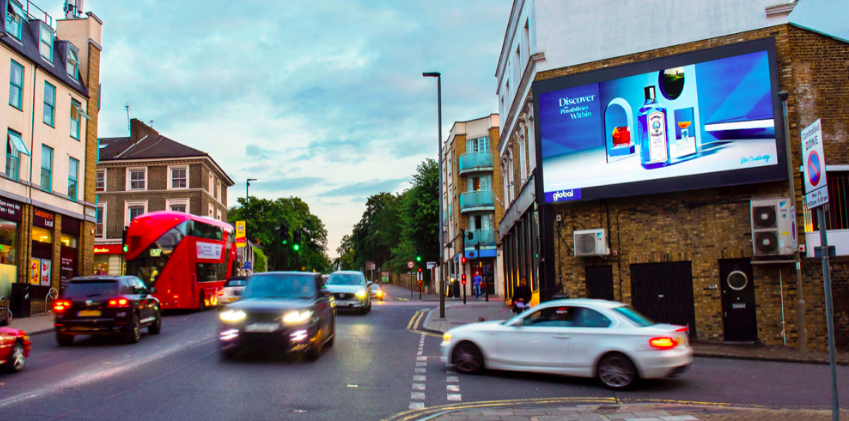
\includegraphics[width=0.7\columnwidth]{./img/DigitalOutdoor.png}
  \caption{Example of a Digital Outdoor, withdrawn from~\cite{digital-outdoor}}%
\label{fig:dig-outdoor}
\end{figure}

Scent market is the art of taking a company's brand identity, marketing messages, target audience and creating a scent that amplifies these values. 
That's because ``a scent has the ability to influence behavior and trigger memories almost instantaneously. When smell is combined with other marketing cues, it can amplify a brand experience and establish a long lasting connection with consumers''~\cite{scent-market}.

Ambient scent uses fragrance to enhance the experience of consumers with different purposes, whereas scents in scent branding are unique to each company's identity.
According to a Samsung study: ``when consumers were exposed to a company scent, shopping time was increased by 26\% and they visited three times more product categories'' ~\cite{scent-stats}.
Also, ``the digital scent technology market is expected to grow from \$1.0 \gls{bn} in 2021 to \$1.5 \gls{bn} by 2026, at a \gls{cagr} of 9.2\%.''~\cite{scent-money}.
%
\begin{figure}[htb!]
\centering
    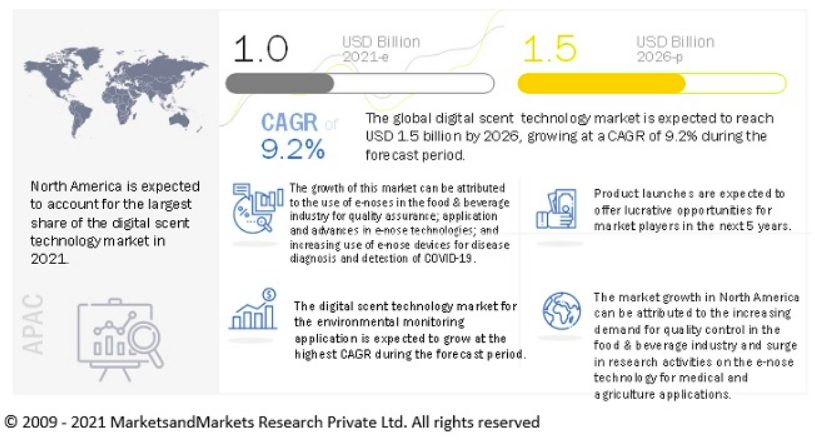
\includegraphics[width=0.9\columnwidth]{./img/scentstats.png}
  \caption{Attractive Opportunities in the Digital Scent Technology Market, withdrawn from~\cite{scent-money}}%
\label{fig:scent-stat}
\end{figure}

The market growth can be attributed to several factors, such as expanding application and advancements in e-nose technologies, increasing use of e-nose devices for disease diagnostic applications, emerging \gls{rd} activities to invent e-nose to sniff out COVID-19, and rising use of e-nose in food industry for quality assurance in production, storage, and display.
%
% Remote material (side by side)
%\begin{figure}[htb!]
%  \centering
  %
%  \begin{subfigure}{.4\textwidth}
%  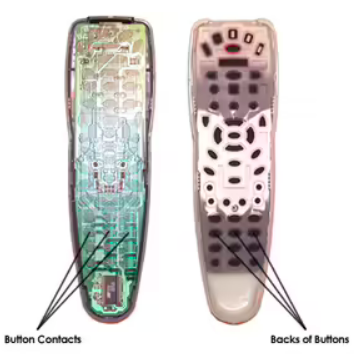
\includegraphics[width=\textwidth]{img/remotematerial1.png}%
  %\caption{KUKA's original position}%
  %\label{fig:ptp-test-orig}
%\end{subfigure}
%
 % \begin{subfigure}{.4\textwidth}
  %  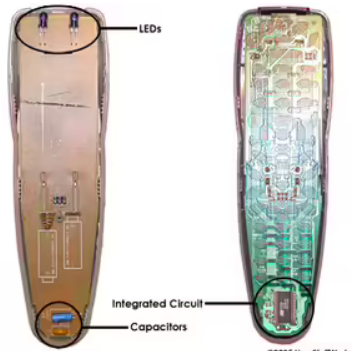
\includegraphics[width=\textwidth]{img/remotematerial2.png}%
%  \caption{KUKA's final position}%
%  \label{fig:ptp-test-final}
%\end{subfigure}
%
%  \caption{TV Remote control bill of materials, withdrawn from~\cite{remotematerial}}%
%  \label{fig:remotemat}
%\end{figure}
%
%
%%% Local Variables:
%%% mode: latex
%%% TeX-master: "../../../dissertation"
%%% End:
